\section{Where space and time meet}

The material derivative describes the \textit{total} experienced change in a scalar quantity, $\bullet$, as \textit{time goes on} \textbf{and} as we \textit{move} across the field of $\bullet$ with fluid velocity $\vec{\bm{V}} = \langle u, \upsilon, w \rangle$.
In this chapter, you can substitute for $\bullet$ any interesting physical quantity that you'd like, such as density, $\rho$, or temperature, $T$.

Pictorially, you may consider a field of $\bullet$ that changes in time and space as presented in Fig.~\ref{fig:material-derivative-example}. In the absence of spatial movement on the $(x,y)$ grid we can still experience change in $\bullet$ in time. Similarly, in the absence of time, we can experience change in $\bullet$ only if we travel on the $(x,y)$ grid and $\bullet$ varies over that grid. With both time and motion present, we will experience a superposition of these two effects and that will be our total experienced change in $\bullet$.
\begin{figure}[H]
\centering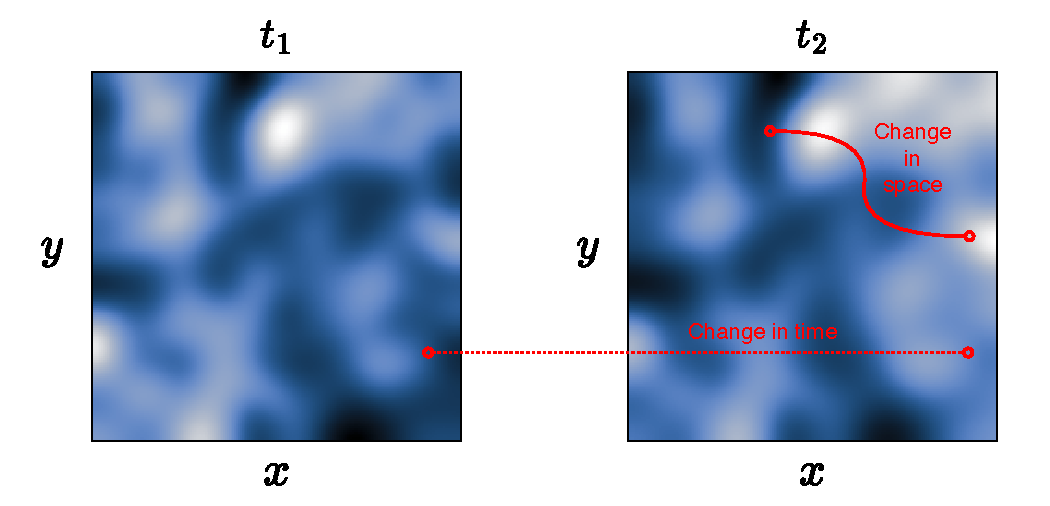
\includegraphics[width=15cm]{material-derivative.pdf}
\caption{A field of some scalar quantity, $\bullet$, that changes in time and space.}			
\label{fig:material-derivative-example}
\end{figure}

In mathematical terms, the material derivative, $\frac{D}{Dt}$, is an operator acting on a scalar, $\bullet$, such that
\begin{equation} \label{eq:material-derivative}
\frac{D \bullet}{D t} \equiv \frac{\partial \bullet}{\partial t} + \vec{\bm{V}} \cdot \nabla \bullet \, .
\end{equation}


But you might rightfully ask: How is the material derivative different from the regular derivative, say $\frac{d}{dt}$ or $\frac{\partial}{\partial t}$? Well, its practical computation isn't mathematically any different from computing regular partial derivatives. Rather, it's simply a special sum of those regular derivatives, such that it accounts for change in time and space \textit{simultaneously}. We can dissect the two terms on the right-hand-side of Eq.~(\ref{eq:material-derivative}) to understand why writing this special sum of partial derivatives makes sense when studying fluid motion.

First, we have $\frac{\partial \bullet}{\partial t}$ which is the plain old\footnote{See Chapter~\ref{chap:changes}.} partial derivative of $\bullet$ with respect to time. It says that at all possible locations in space, and at any one location, the quantity $\bullet$ can evolve in time. One example of such quantity is temperature. Even if we remain stationary in a specific location, say in a corner of a room, we can still experience change in temperature because our room might be heated (or cooled) and the temperature in our little corner changes in time because of that. The term $\frac{\partial \bullet}{\partial t}$ gives us a recipe for \textit{how} that temperature changes in time in every location of the room.

Second, we have $\vec{\bm{V}} \cdot \nabla \bullet$, that is, a gradient vector, $\nabla \bullet = \langle \frac{\partial \bullet}{\partial x}, \frac{\partial \bullet}{\partial y}, \frac{\partial \bullet}{\partial z} \rangle$, dotted with the velocity vector, $\vec{\bm{V}}$. At this point, you might remind yourself of the intuition behind taking a dot product between two vectors from Fig.~\ref{fig:circulation-dot-product}. The gradient of $\bullet$ is a vector field that describes directions in which $\bullet$ varies. If, and only if, your own movement is aligned (at least to some extent) with the direction of $\bullet$'s gradient, you will experience a change in quantity $\bullet$. Otherwise, if you walk along an isocurve of $\bullet$, you will not experience any change in $\bullet$.

In other words, the first term on the right-hand-side of Eq.~(\ref{eq:material-derivative}) describes how we will experience change in $\bullet$ in the absence of our motion through the field. The second term describes how we will experience additional change due to moving around through the field. The material derivative is a neat superposition of these two factors for why $\bullet$ can change. It is also a shorthand for describing change in $\bullet$ in a moving fluid and it has been created because this set is frequently used in fluid dynamics related equations. Writing it in short as $\frac{D}{D t}$ simply makes life easier.

\begin{mdframed}[style=exercise-frame]

\subsection*{Searching for more?}

You can find a great intuitive description of a material derivative in Chapter~3, \S3.5 of the \textit{Transport Phenomena} textbook by Bird, Stewart \& Lightfoot \cite{bird2002transport}. They delineate differences between various derivatives on the example of following fish in a Mississippi river (or St. Croix River in the newer version of the textbook!).

\end{mdframed}

Finally, I would like to present two more ways of writing Eq.~(\ref{eq:material-derivative}) just to expose you to other possible notations that you might encounter in textbooks. 
In the most general 3D case, where $\vec{\bm{V}} = \langle u, \upsilon, w \rangle$, we can expand the dot product terms to obtain:
\begin{equation} \label{eq:material-derivative-full}
\frac{D \bullet}{D t} \equiv \frac{\partial \bullet}{\partial t} + u \frac{\partial \bullet}{\partial x} + \upsilon \frac{\partial \bullet}{\partial y} + w \frac{\partial \bullet}{\partial z} \, .
\end{equation}
A yet another way of writing the equation above that you might sometimes encounter is the following:
\begin{equation} \label{eq:material-derivative-ein stein}
\frac{D \bullet}{D t} \equiv \frac{\partial \bullet}{\partial t} + V_i \frac{\partial \bullet}{\partial i} \, .
\end{equation}
This way of writing Eq.~(\ref{eq:material-derivative-full}) is using the Einstein notation, where it is implied that you should substitute for the dummy index $i$ every possible spatial dimension, \textit{i.e.}, $x$, $y$, and $z$, and, as you substitute, you also sum up all the terms that form for each possible $i$.

\section{Pause and ponder}

Let's look at some alternate ways to describe change in both space and time and see why they wouldn't be equally useful as Eq.~(\ref{eq:material-derivative})! Suppose I present you with the following quantity:
\begin{equation} \label{eq:all-derivatives}
\frac{\partial \bullet}{\partial t} + \frac{\partial \bullet}{\partial x} + \frac{\partial \bullet}{\partial y} + \frac{\partial \bullet}{\partial z} \, .
\end{equation}
How is that quantity different from the definition of the material derivative? In other words, what does the dot product with the velocity vector change in how we described change in space in Eq.~(\ref{eq:material-derivative-full})?

The velocity vector is not our independent motion through the field of $\bullet$. It is our motion when carried by the fluid flow.


This discussion tells us something deeper about the philosophy of describing fluid motion. Material derivative is inherently tied to the continuum assumption in fluid dynamics.

In essence, the material derivative describes our experience change in $\bullet$ because of our motion with the fluid velocity, even though the change in $\bullet$ might happen precisely \textit{due to} fluid motion. Think about the fluid density, $\rho$, which can change due to local movement of fluid from one location to the next.



